% Options for packages loaded elsewhere
\PassOptionsToPackage{unicode}{hyperref}
\PassOptionsToPackage{hyphens}{url}
%
\documentclass[
]{article}
\usepackage{lmodern}
\usepackage{amssymb,amsmath}
\usepackage{ifxetex,ifluatex}
\ifnum 0\ifxetex 1\fi\ifluatex 1\fi=0 % if pdftex
  \usepackage[T1]{fontenc}
  \usepackage[utf8]{inputenc}
  \usepackage{textcomp} % provide euro and other symbols
\else % if luatex or xetex
  \usepackage{unicode-math}
  \defaultfontfeatures{Scale=MatchLowercase}
  \defaultfontfeatures[\rmfamily]{Ligatures=TeX,Scale=1}
\fi
% Use upquote if available, for straight quotes in verbatim environments
\IfFileExists{upquote.sty}{\usepackage{upquote}}{}
\IfFileExists{microtype.sty}{% use microtype if available
  \usepackage[]{microtype}
  \UseMicrotypeSet[protrusion]{basicmath} % disable protrusion for tt fonts
}{}
\makeatletter
\@ifundefined{KOMAClassName}{% if non-KOMA class
  \IfFileExists{parskip.sty}{%
    \usepackage{parskip}
  }{% else
    \setlength{\parindent}{0pt}
    \setlength{\parskip}{6pt plus 2pt minus 1pt}}
}{% if KOMA class
  \KOMAoptions{parskip=half}}
\makeatother
\usepackage{xcolor}
\IfFileExists{xurl.sty}{\usepackage{xurl}}{} % add URL line breaks if available
\IfFileExists{bookmark.sty}{\usepackage{bookmark}}{\usepackage{hyperref}}
\hypersetup{
  pdftitle={Visualizing mobloc},
  pdfauthor={Martijn Tennekes},
  hidelinks,
  pdfcreator={LaTeX via pandoc}}
\urlstyle{same} % disable monospaced font for URLs
\usepackage[margin=1in]{geometry}
\usepackage{color}
\usepackage{fancyvrb}
\newcommand{\VerbBar}{|}
\newcommand{\VERB}{\Verb[commandchars=\\\{\}]}
\DefineVerbatimEnvironment{Highlighting}{Verbatim}{commandchars=\\\{\}}
% Add ',fontsize=\small' for more characters per line
\usepackage{framed}
\definecolor{shadecolor}{RGB}{248,248,248}
\newenvironment{Shaded}{\begin{snugshade}}{\end{snugshade}}
\newcommand{\AlertTok}[1]{\textcolor[rgb]{0.94,0.16,0.16}{#1}}
\newcommand{\AnnotationTok}[1]{\textcolor[rgb]{0.56,0.35,0.01}{\textbf{\textit{#1}}}}
\newcommand{\AttributeTok}[1]{\textcolor[rgb]{0.77,0.63,0.00}{#1}}
\newcommand{\BaseNTok}[1]{\textcolor[rgb]{0.00,0.00,0.81}{#1}}
\newcommand{\BuiltInTok}[1]{#1}
\newcommand{\CharTok}[1]{\textcolor[rgb]{0.31,0.60,0.02}{#1}}
\newcommand{\CommentTok}[1]{\textcolor[rgb]{0.56,0.35,0.01}{\textit{#1}}}
\newcommand{\CommentVarTok}[1]{\textcolor[rgb]{0.56,0.35,0.01}{\textbf{\textit{#1}}}}
\newcommand{\ConstantTok}[1]{\textcolor[rgb]{0.00,0.00,0.00}{#1}}
\newcommand{\ControlFlowTok}[1]{\textcolor[rgb]{0.13,0.29,0.53}{\textbf{#1}}}
\newcommand{\DataTypeTok}[1]{\textcolor[rgb]{0.13,0.29,0.53}{#1}}
\newcommand{\DecValTok}[1]{\textcolor[rgb]{0.00,0.00,0.81}{#1}}
\newcommand{\DocumentationTok}[1]{\textcolor[rgb]{0.56,0.35,0.01}{\textbf{\textit{#1}}}}
\newcommand{\ErrorTok}[1]{\textcolor[rgb]{0.64,0.00,0.00}{\textbf{#1}}}
\newcommand{\ExtensionTok}[1]{#1}
\newcommand{\FloatTok}[1]{\textcolor[rgb]{0.00,0.00,0.81}{#1}}
\newcommand{\FunctionTok}[1]{\textcolor[rgb]{0.00,0.00,0.00}{#1}}
\newcommand{\ImportTok}[1]{#1}
\newcommand{\InformationTok}[1]{\textcolor[rgb]{0.56,0.35,0.01}{\textbf{\textit{#1}}}}
\newcommand{\KeywordTok}[1]{\textcolor[rgb]{0.13,0.29,0.53}{\textbf{#1}}}
\newcommand{\NormalTok}[1]{#1}
\newcommand{\OperatorTok}[1]{\textcolor[rgb]{0.81,0.36,0.00}{\textbf{#1}}}
\newcommand{\OtherTok}[1]{\textcolor[rgb]{0.56,0.35,0.01}{#1}}
\newcommand{\PreprocessorTok}[1]{\textcolor[rgb]{0.56,0.35,0.01}{\textit{#1}}}
\newcommand{\RegionMarkerTok}[1]{#1}
\newcommand{\SpecialCharTok}[1]{\textcolor[rgb]{0.00,0.00,0.00}{#1}}
\newcommand{\SpecialStringTok}[1]{\textcolor[rgb]{0.31,0.60,0.02}{#1}}
\newcommand{\StringTok}[1]{\textcolor[rgb]{0.31,0.60,0.02}{#1}}
\newcommand{\VariableTok}[1]{\textcolor[rgb]{0.00,0.00,0.00}{#1}}
\newcommand{\VerbatimStringTok}[1]{\textcolor[rgb]{0.31,0.60,0.02}{#1}}
\newcommand{\WarningTok}[1]{\textcolor[rgb]{0.56,0.35,0.01}{\textbf{\textit{#1}}}}
\usepackage{graphicx,grffile}
\makeatletter
\def\maxwidth{\ifdim\Gin@nat@width>\linewidth\linewidth\else\Gin@nat@width\fi}
\def\maxheight{\ifdim\Gin@nat@height>\textheight\textheight\else\Gin@nat@height\fi}
\makeatother
% Scale images if necessary, so that they will not overflow the page
% margins by default, and it is still possible to overwrite the defaults
% using explicit options in \includegraphics[width, height, ...]{}
\setkeys{Gin}{width=\maxwidth,height=\maxheight,keepaspectratio}
% Set default figure placement to htbp
\makeatletter
\def\fps@figure{htbp}
\makeatother
\setlength{\emergencystretch}{3em} % prevent overfull lines
\providecommand{\tightlist}{%
  \setlength{\itemsep}{0pt}\setlength{\parskip}{0pt}}
\setcounter{secnumdepth}{-\maxdimen} % remove section numbering

\title{Visualizing mobloc}
\author{Martijn Tennekes}
\date{2020-09-18}

\begin{document}
\maketitle

The \textbf{mobloc} package is used to approximate geographic location
given the connection between a mobile device and the cell (an antenna
may contain multiple cells). This is done by a physical model of signal
strength and a Bayesian method to estimate the location of mobile
devices. The latter is done by applying Bayes' formula

\(P(g|a) \sim P(g)P(a|g)\)

where

\begin{itemize}
\tightlist
\item
  \(P(g|a)\) is the \emph{posterior} probability that a device is
  located in grid tile \(g\) given that it is connected to cell \(a\),
\item
  \$P(g) is the \emph{prior} probability that a device is located in
  grid tile \(g\). The most simple model is to set it to a constant
  value. Alternatively, external data sources such as land use can be
  used.
\item
  \(P(a|g)\) is the \emph{likelihood} probability, which is the
  probability that a device is connected to cell \(a\) given that is it
  located in grid tile \(g\). For the computation of these probability,
  mobloc offers two methods: the first uses Voronoi, which assumes that
  a device will always be connected to the nearest cell, and the second
  uses the signal strength model. In a wider context, these
  probabilities are also called \emph{event location} {[}3{]}.
\end{itemize}

These methods are described in detail in {[}1{]}. The implementation is
described in the documentation of the \textbf{mobloc} package {[}2{]}.

\hypertarget{processing-example-data-in-mobloc}{%
\subsection{Processing example data in
mobloc}\label{processing-example-data-in-mobloc}}

The \textbf{mobloc} package contains fictional \textbf{cellplan} dataset
called \texttt{ZL\_cellplan}. A cellplan is a dataset that contains the
locations and physical properties of the cells from a certain MNO. The
cells in \texttt{ZL\_cellplan} are fictionally placed in the region of
Zuid-Limburg, which is NUTS region NL423. Besides the cellplan, other
datasets that are contained in \textbf{mobloc} are the municipality
polygons for Zuid-Limburg \texttt{ZL\_muni}, the elevation data
\texttt{ZL\_elevation}, and land use data \texttt{ZL\_landuse}.

These datasets area loaded as follows.

\begin{Shaded}
\begin{Highlighting}[]
\KeywordTok{library}\NormalTok{(mobloc)}
\KeywordTok{data}\NormalTok{(}\StringTok{"ZL_cellplan"}\NormalTok{, }\StringTok{"ZL_muni"}\NormalTok{, }\StringTok{"ZL_elevation"}\NormalTok{, }\StringTok{"ZL_landuse"}\NormalTok{)}
\end{Highlighting}
\end{Shaded}

\texttt{ZL\_cellplan} and \texttt{ZL\_muni} are \textbf{sf} {[}4{]}
objects of points and polygons respectively. The objects
\texttt{ZL\_elevation} and \texttt{ZL\_landuse} are \textbf{raster}
{[}5{]} objects.

The following code processes these input datasets.

\begin{Shaded}
\begin{Highlighting}[]
\CommentTok{# set parameters}
\NormalTok{ZL_param <-}\StringTok{ }\KeywordTok{mobloc_param}\NormalTok{()}

\CommentTok{# create environment layer (needed to calculate path loss exponent (ple))}
\NormalTok{ZL_envir <-}\StringTok{ }\KeywordTok{combine_raster_layers}\NormalTok{(ZL_landuse, }\DataTypeTok{weights =} \KeywordTok{c}\NormalTok{(}\DecValTok{1}\NormalTok{, }\DecValTok{1}\NormalTok{, }\DecValTok{1}\NormalTok{, }\DecValTok{0}\NormalTok{, }\DecValTok{0}\NormalTok{))}

\CommentTok{# validate cellplan}
\NormalTok{ZL_cellplan <-}\StringTok{ }\KeywordTok{validate_cellplan}\NormalTok{(ZL_cellplan, }\DataTypeTok{param =}\NormalTok{ ZL_param, }\DataTypeTok{region =}\NormalTok{ ZL_muni,}
    \DataTypeTok{envir =}\NormalTok{ ZL_envir, }\DataTypeTok{elevation =}\NormalTok{ ZL_elevation)}
\CommentTok{#> Variable 'W' is missing. These have been imputed with the parameters 'W' and 'W_small' for normal and small cells respectively.}
\CommentTok{#> Variable 'range' is missing. These have been imputed with the parameters 'range' and 'range_small' for normal and small cells respectively.}
\CommentTok{#> Path loss exponent ('ple') values updated with envir object}
\CommentTok{#> The cellplan has been made valid}

\CommentTok{# create raster}
\NormalTok{ZL_bbox <-}\StringTok{ }\NormalTok{sf}\OperatorTok{::}\KeywordTok{st_bbox}\NormalTok{(}\KeywordTok{c}\NormalTok{(}\DataTypeTok{xmin =} \DecValTok{4012000}\NormalTok{, }\DataTypeTok{ymin =} \DecValTok{3077000}\NormalTok{, }\DataTypeTok{xmax =} \DecValTok{4048000}\NormalTok{, }\DataTypeTok{ymax =} \DecValTok{3117000}\NormalTok{),}
    \DataTypeTok{crs =}\NormalTok{ sf}\OperatorTok{::}\KeywordTok{st_crs}\NormalTok{(}\DecValTok{3035}\NormalTok{))}
\NormalTok{ZL_raster <-}\StringTok{ }\KeywordTok{create_raster}\NormalTok{(ZL_bbox)}

\CommentTok{# compute the signal strength model}
\NormalTok{ZL_strength <-}\StringTok{ }\KeywordTok{compute_sig_strength}\NormalTok{(}\DataTypeTok{cp =}\NormalTok{ ZL_cellplan, }\DataTypeTok{raster =}\NormalTok{ ZL_raster,}
    \DataTypeTok{elevation =}\NormalTok{ ZL_elevation, }\DataTypeTok{param =}\NormalTok{ ZL_param)}
\CommentTok{#> Determining coverage area per cell}
\CommentTok{#> Determine signal strength per cell for raster tiles inside coverage area}
\CommentTok{#> Creating data.frame and compute pag values}

\CommentTok{# create likelihoods (event locations)}
\NormalTok{ZL_strength_llh <-}\StringTok{ }\KeywordTok{create_strength_llh}\NormalTok{(ZL_strength, }\DataTypeTok{param =}\NormalTok{ ZL_param)}
\NormalTok{ZL_voronoi_llh <-}\StringTok{ }\KeywordTok{create_voronoi_llh}\NormalTok{(ZL_cellplan, ZL_raster)}

\CommentTok{# create priors}
\NormalTok{ZL_uniform_prior <-}\StringTok{ }\KeywordTok{create_uniform_prior}\NormalTok{(ZL_raster)}
\NormalTok{ZL_network_prior <-}\StringTok{ }\KeywordTok{create_network_prior}\NormalTok{(ZL_strength, ZL_raster)}
\NormalTok{ZL_landuse_prior <-}\StringTok{ }\KeywordTok{create_prior}\NormalTok{(ZL_landuse, }\DataTypeTok{weights =} \KeywordTok{c}\NormalTok{(}\DecValTok{1}\NormalTok{, }\DecValTok{1}\NormalTok{, }\FloatTok{.1}\NormalTok{, }\DecValTok{0}\NormalTok{, }\FloatTok{.5}\NormalTok{))}

\CommentTok{# create composite prior: half network, half lansuse}
\NormalTok{ZL_composite_prior <-}\StringTok{ }\KeywordTok{create_prior}\NormalTok{(ZL_network_prior, ZL_landuse_prior, }\DataTypeTok{weights =} \KeywordTok{c}\NormalTok{(}\FloatTok{0.5}\NormalTok{, }\FloatTok{0.5}\NormalTok{))}

\CommentTok{# caculate the posterior distributions}
\NormalTok{ZL_posterior <-}\StringTok{ }\KeywordTok{calculate_posterior}\NormalTok{(}\DataTypeTok{prior =}\NormalTok{ ZL_composite_prior, }
    \DataTypeTok{llh =}\NormalTok{ ZL_strength_llh, }\DataTypeTok{raster =}\NormalTok{ ZL_raster)}
\end{Highlighting}
\end{Shaded}

This code is explained in the documentation of the \textbf{mobloc}
package. The most important objects are:

\begin{itemize}
\tightlist
\item
  \texttt{ZL\_param}, a list that contains all the parameters used in
  \textbf{mobloc}, e.g.~the default physical properties of the cells.
\item
  \texttt{ZL\_raster}, a \texttt{raster} object that contains the
  geospatial information of the grid tiles, e.g.~their spatial position
  and the resolution.
\item
  \texttt{ZL\_strength}, a \texttt{data.table} object that contains the
  signal strength in \texttt{dBm} and the signal dominance (called
  \texttt{s}) per grid tile,
\item
  \texttt{ZL\_xxx\_llh}, \texttt{data.table} objects that contain the
  likelihood probabilities (event locations) per cell. This probability
  is called \texttt{pag}, which stands for \texttt{p(a\textbar{}g)},
  which is the probability that a device is connected to cell
  \texttt{a}, given that it is located in grid tile \texttt{g}.
\item
  \texttt{ZL\_xxx\_prior}, \texttt{raster} objects in the same
  resolution as \texttt{ZL\_raster}, that contain prior information.
  This probability is called \texttt{pg}, which stands for
  \texttt{p(g)}, the probability that a device is located in grid tile
  \texttt{g}.
\item
  \texttt{ZL\_posterior}, a \texttt{data.table} that contains the
  posterior probabilities. This probability is called \texttt{pga},
  which stands for \texttt{p(g\textbar{}a)}, which is the probability
  that a device is located in grid tile \texttt{g}, given that it is
  connected to cell \texttt{a}.
\end{itemize}

\hypertarget{visualization-of-mobloc-parameters}{%
\subsection{Visualization of mobloc
parameters}\label{visualization-of-mobloc-parameters}}

\begin{Shaded}
\begin{Highlighting}[]
\KeywordTok{library}\NormalTok{(mobvis)}
\end{Highlighting}
\end{Shaded}

The following function starts a dashboard that examines the parameters
used in mobloc.

\begin{Shaded}
\begin{Highlighting}[]
\KeywordTok{setup_sig_strength_model}\NormalTok{()}
\end{Highlighting}
\end{Shaded}

This tool shows the signal strength model for one cell.

The left hand side panel shows the settings, which are by default set to
values of the list we created with \texttt{mobloc\_param()}. The plots
on the right hand side shows the propagation results. The heatmap on the
top right shows the top view of the signal strength of the cell. The
direction of directional cells is east in this plot. The four plots
below the heatmap can be reproduced with the following single function
calls.

The function \texttt{distance\_plot} plots the relation between signal
strength (in dBm) and distance in the propagation direction of the cell.
This depends on the cell power in watt (\texttt{W}) and the path loss
exponent (\texttt{ple}) which models how well the signal propagates (2
is free space, 4 is urban area, and is inside buildings).

\begin{Shaded}
\begin{Highlighting}[]
\KeywordTok{distance_plot}\NormalTok{(}\DataTypeTok{W =} \DecValTok{4}\NormalTok{, }\DataTypeTok{ple =} \DecValTok{4}\NormalTok{, }\DataTypeTok{range =} \DecValTok{2000}\NormalTok{)}
\end{Highlighting}
\end{Shaded}

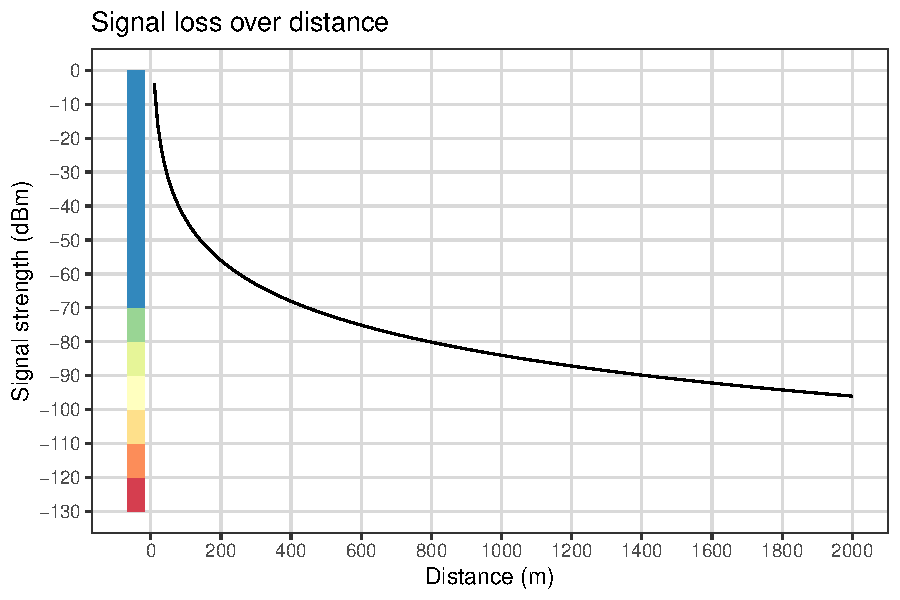
\includegraphics{mobvis-mobloc_files/figure-latex/unnamed-chunk-5-1.pdf}

The color codes on the y-axis resemble how well the signal is for mobile
communication. This will be further discussed later on.

The function \texttt{signal\_dominance\_plot} plots the modeled relation
between signal strength (in dBm) and the signal dominance (s).

\begin{Shaded}
\begin{Highlighting}[]
\KeywordTok{signal_dominance_plot}\NormalTok{(}\DataTypeTok{midpoint =} \DecValTok{-90}\NormalTok{, }\DataTypeTok{steepness =} \FloatTok{0.5}\NormalTok{)}
\end{Highlighting}
\end{Shaded}

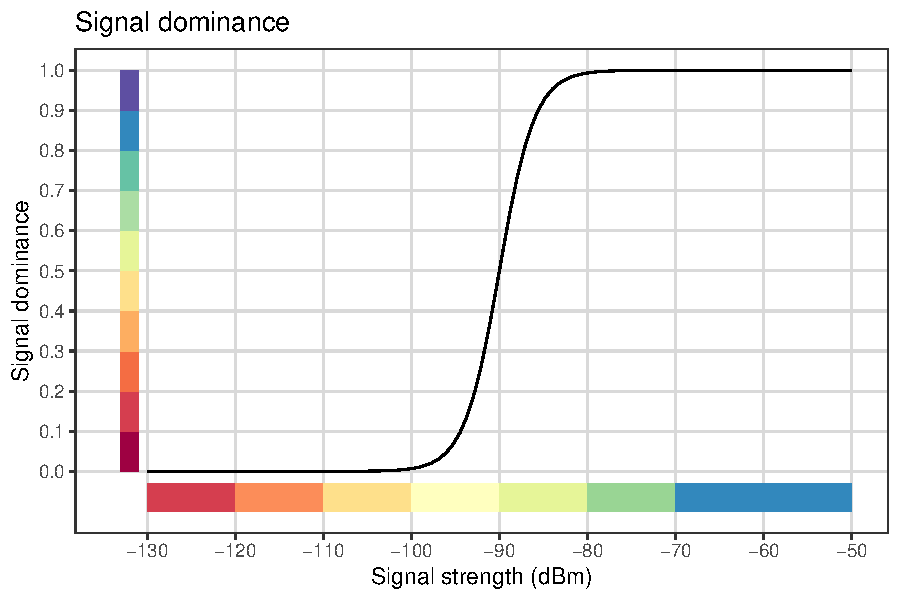
\includegraphics{mobvis-mobloc_files/figure-latex/unnamed-chunk-6-1.pdf}

Signal dominance can be interpreted as the quality of a connection
between device and mobile phone, or in other words, how attractive it is
to make create connection. It is based on the assumption that for a
mobile phone network, it is not important whether the connection is good
(say -90 dBm) or extreme good (say -70 dBm). When there are multiple
cells to choose from, the current capacity is much more important.
Likewise, if there is only one available cell for a device to connect to
at a certain location, the network will do that, no matter whether the
connection is fair (say -100 dBm) or bad (say -120 dBm). This has been
modeled by flattening both tails of the distribution. A logistic
function has been applied to do this {[}1{]}, where its parameters are
midpoint and steepness.

The function \texttt{radiation\_plot} plots the modeled radiation
pattern from the cell. The radiation pattern indicates how much signal
loss there is in the azimuth plane (top view perpendicular to the
propagation direction), and the elevation plane (side view perpendicular
to the propagation direction). The black contour lines indicate the
signal loss as a function of the offset angle. The red points are the
-3dB points, i.e.~the angle at which the signal loss is 3 dB. The three
parameters for this pattern are \texttt{type} which indicated whether it
is applied to the azimuth (\texttt{"a"}) or elevation (\texttt{"e"})
place, \texttt{beam\_width}, which specifies the angle at which the
signal loss is 3 dB (so the angle between the red points in the
diagram), and \texttt{db\_back} which defines the signall loss the the
angle in the opposite direction of the propagation direction.

\begin{Shaded}
\begin{Highlighting}[]
\KeywordTok{radiation_plot}\NormalTok{(}\DataTypeTok{type =} \StringTok{"a"}\NormalTok{, }\DataTypeTok{beam_width =} \DecValTok{60}\NormalTok{, }\DataTypeTok{db_back =} \DecValTok{-30}\NormalTok{)}
\KeywordTok{radiation_plot}\NormalTok{(}\DataTypeTok{type =} \StringTok{"e"}\NormalTok{, }\DataTypeTok{beam_width =} \DecValTok{10}\NormalTok{, }\DataTypeTok{db_back =} \DecValTok{-30}\NormalTok{)}
\end{Highlighting}
\end{Shaded}

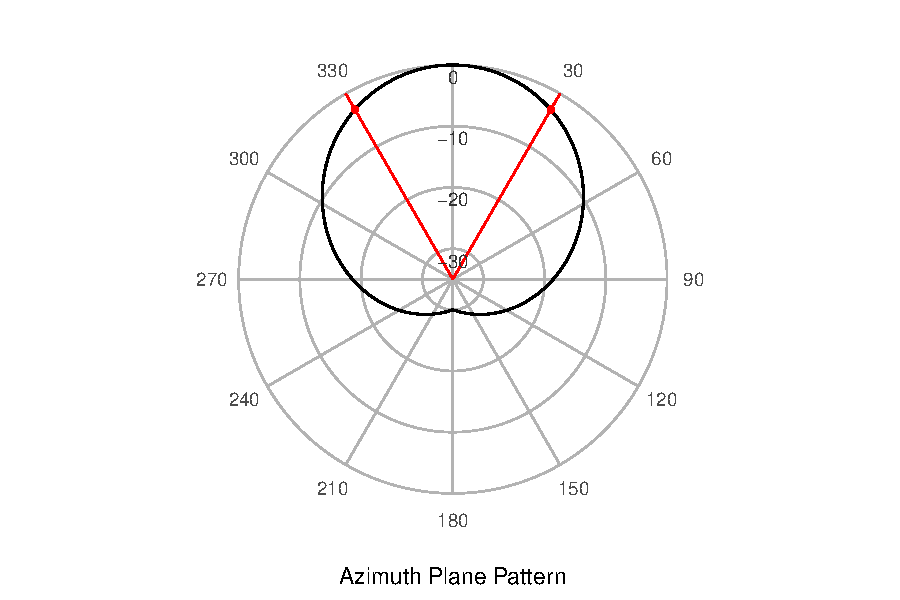
\includegraphics[width=0.46\linewidth]{mobvis-mobloc_files/figure-latex/unnamed-chunk-7-1}
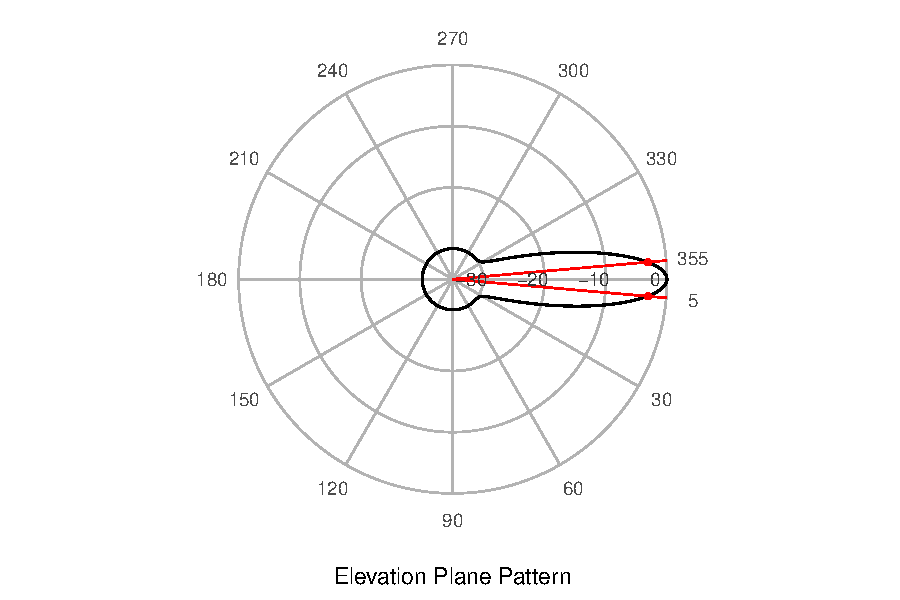
\includegraphics[width=0.46\linewidth]{mobvis-mobloc_files/figure-latex/unnamed-chunk-7-2}

\hypertarget{visualization-of-the-mobloc-output}{%
\subsection{Visualization of the mobloc
output}\label{visualization-of-the-mobloc-output}}

The dashboard that examines the processed data from \textbf{mobloc} can
be called as follows:

\begin{Shaded}
\begin{Highlighting}[]
\CommentTok{# explore the results}
\KeywordTok{explore_mobloc}\NormalTok{(}
    \DataTypeTok{cp =}\NormalTok{ ZL_cellplan, }
    \DataTypeTok{raster =}\NormalTok{ ZL_raster, }
    \DataTypeTok{strength =}\NormalTok{ ZL_strength,}
    \DataTypeTok{priorlist =} \KeywordTok{list}\NormalTok{(}\DataTypeTok{landuse =}\NormalTok{ ZL_landuse_prior, }\DataTypeTok{network =}\NormalTok{ ZL_network_prior, }\DataTypeTok{uniform =}\NormalTok{ ZL_uniform_prior),}
    \DataTypeTok{llhlist =} \KeywordTok{list}\NormalTok{(}\DataTypeTok{Strength =}\NormalTok{ ZL_strength_llh, }\DataTypeTok{Voronoi =}\NormalTok{ ZL_voronoi_llh),}
    \DataTypeTok{param =}\NormalTok{ ZL_param)}
\end{Highlighting}
\end{Shaded}

In the left-hand-side panel, the user is able to select which raster
variable is shown on the map. The options are listed on the left-most
column. They are: signal strength (dBm), signal dominance (s), best
server map, prior, likelihood, and posterior. For each of them there is
a stand-alone function which will be shown and described below. The
first option, called ``Selection'' determines whether the data is shown
for all cells or one single cell. In the former case, the maximum number
per grid tile is shown. For instance, if the signal strength in dBm is
selected for all cells, the color of a grid tile represents the maximum
signal strength.

The second column, called ``Module Setup'' configures the prior, the
likelihood, the posterior (which uses the chosen prior and likelihood),
and whether Timing Advance is used. In the other tab panel, called
``Cell data'', cellplan data per cell is shown in a table.

\hypertarget{signal-strength-and-signal-dominance}{%
\subsubsection{Signal strength and signal
dominance}\label{signal-strength-and-signal-dominance}}

The function \texttt{map\_sig\_strength} is used to map the signal
strength or dominance. Which of these two will be shown depends on the
\texttt{type} argument.

\begin{Shaded}
\begin{Highlighting}[]
\KeywordTok{map_sig_strength}\NormalTok{(}\DataTypeTok{rst =}\NormalTok{ ZL_raster, }
                 \DataTypeTok{dt =}\NormalTok{ ZL_strength, }
                 \DataTypeTok{cp =}\NormalTok{ ZL_cellplan, }
                 \DataTypeTok{cells =} \StringTok{"BEE_150_N1"}\NormalTok{, }
                 \DataTypeTok{region =}\NormalTok{ ZL_muni, }
                 \DataTypeTok{type =} \StringTok{"dBm"}\NormalTok{, }
                 \DataTypeTok{interactive =} \OtherTok{FALSE}\NormalTok{)}
\KeywordTok{map_sig_strength}\NormalTok{(}\DataTypeTok{rst =}\NormalTok{ ZL_raster, }
                 \DataTypeTok{dt =}\NormalTok{ ZL_strength, }
                 \DataTypeTok{cp =}\NormalTok{ ZL_cellplan, }
                 \DataTypeTok{cells =} \StringTok{"BEE_150_N1"}\NormalTok{, }
                 \DataTypeTok{region =}\NormalTok{ ZL_muni, }
                 \DataTypeTok{type =} \StringTok{"dBm"}\NormalTok{, }
                 \DataTypeTok{interactive =} \OtherTok{FALSE}\NormalTok{, }
                 \DataTypeTok{settings =} \KeywordTok{mobvis_settings}\NormalTok{(}\DataTypeTok{use_classes =} \OtherTok{FALSE}\NormalTok{))}
\KeywordTok{map_sig_strength}\NormalTok{(}\DataTypeTok{rst =}\NormalTok{ ZL_raster, }
                 \DataTypeTok{dt =}\NormalTok{ ZL_strength, }
                 \DataTypeTok{cp =}\NormalTok{ ZL_cellplan, }
                 \DataTypeTok{cells =} \StringTok{"BEE_150_N1"}\NormalTok{, }
                 \DataTypeTok{region =}\NormalTok{ ZL_muni, }
                 \DataTypeTok{type =} \StringTok{"s"}\NormalTok{, }
                 \DataTypeTok{interactive =} \OtherTok{FALSE}\NormalTok{)}
\KeywordTok{map_sig_strength}\NormalTok{(}\DataTypeTok{rst =}\NormalTok{ ZL_raster, }
                 \DataTypeTok{dt =}\NormalTok{ ZL_strength, }
                 \DataTypeTok{cp =}\NormalTok{ ZL_cellplan, }
                 \DataTypeTok{cells =} \StringTok{"BEE_150_N1"}\NormalTok{, }
                 \DataTypeTok{region =}\NormalTok{ ZL_muni, }
                 \DataTypeTok{type =} \StringTok{"s"}\NormalTok{, }
                 \DataTypeTok{interactive =} \OtherTok{FALSE}\NormalTok{, }
                 \DataTypeTok{settings =} \KeywordTok{mobvis_settings}\NormalTok{(}\DataTypeTok{use_classes =} \OtherTok{FALSE}\NormalTok{))}
\end{Highlighting}
\end{Shaded}

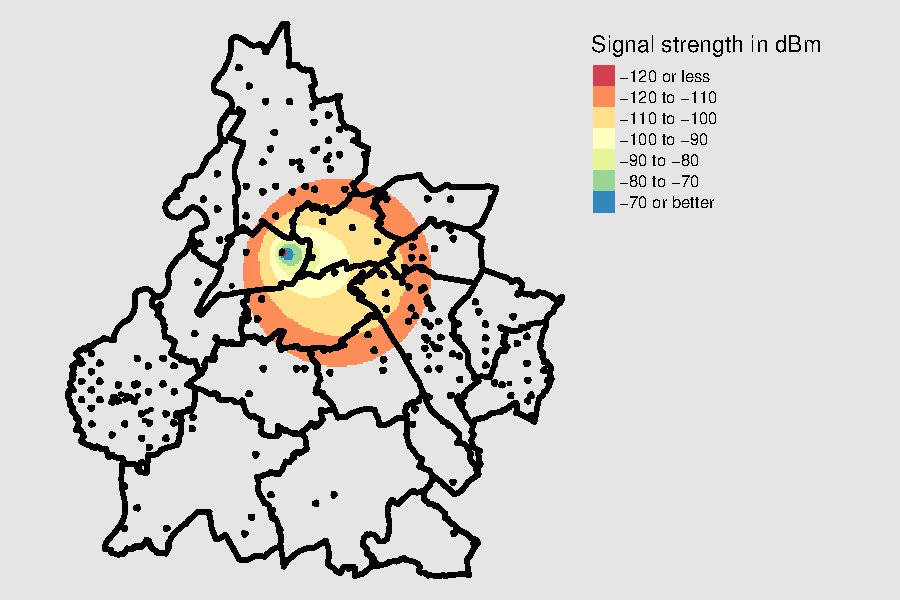
\includegraphics[width=0.46\linewidth]{mobvis-mobloc_files/figure-latex/unnamed-chunk-9-1}
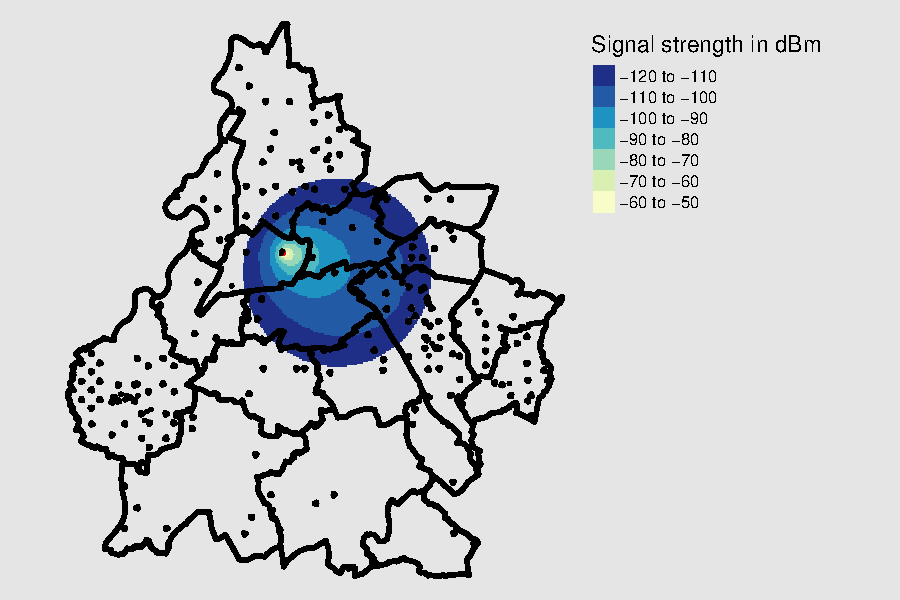
\includegraphics[width=0.46\linewidth]{mobvis-mobloc_files/figure-latex/unnamed-chunk-9-2}
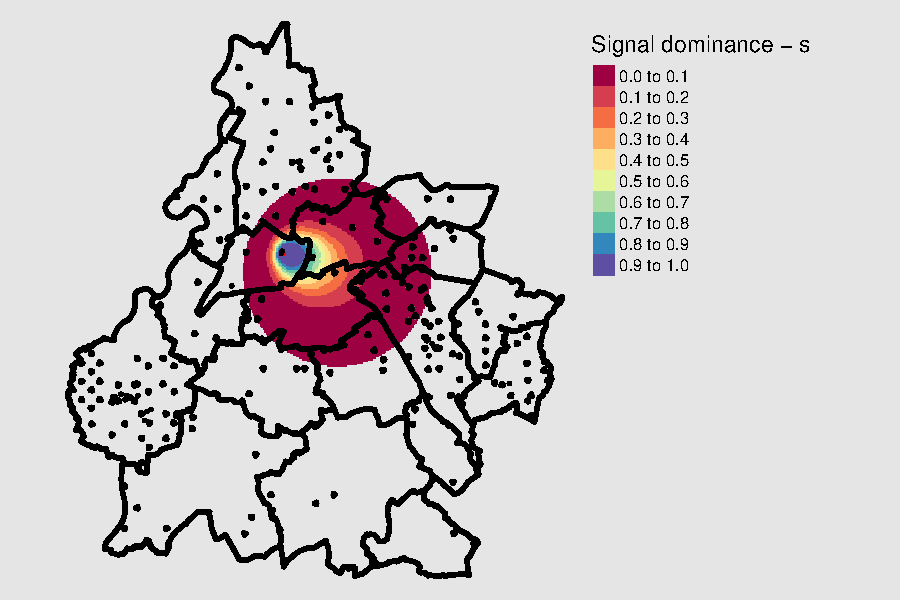
\includegraphics[width=0.46\linewidth]{mobvis-mobloc_files/figure-latex/unnamed-chunk-9-3}
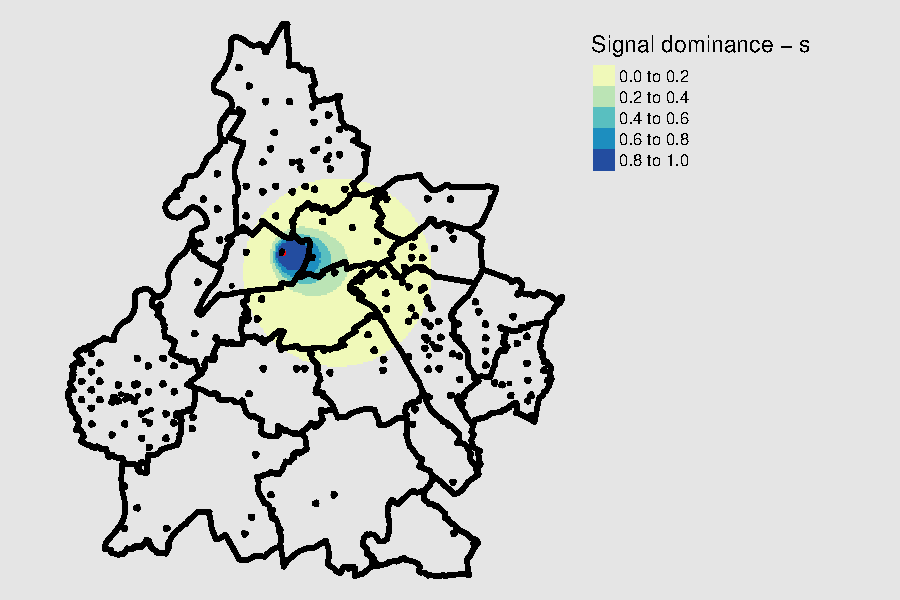
\includegraphics[width=0.46\linewidth]{mobvis-mobloc_files/figure-latex/unnamed-chunk-9-4}

The function \texttt{mobvis\_settings()} returns a list that contains
settings for the plots drawn by \textbf{mobvis}. For instance default
color palettes, titles, and whether the plot is static (such as shown
here) or interactive (shown in the screenshot of the dashboard tool).
The function \texttt{mobvis\_settings\_interactive()} returns the same
list, with a few different values, which are aimed for interactive
plots. For instance, the cells are by deafult drawn in black in statis
maps and yellow with a black border in interactive maps. The function
\texttt{mobvis\_settings\_animation()} contains settings for animations,
which are described in the other vigentte.

As for signal strength and signal dominance, by default a diverging
color palette is shown, from red via yellow to blue, which qualifies the
signal strength/dominance as more or less as follows: red is bad, orange
is poor, yellow is fair, green is good, and blue is excellent. The
mappings (so which values are bad, poor, etc.) can be adjusted via
\texttt{mobvis\_settings}. There is also a setting that disables these
classes, which is in the maps on the right hand side.

\hypertarget{prior-likelihood-and-posterior}{%
\subsubsection{Prior, likelihood and
posterior}\label{prior-likelihood-and-posterior}}

The prior, likelihood and posterior can be shown with the functions
\texttt{map\_pg}, \texttt{map\_pag}, and \texttt{map\_pga} respectively.

\begin{Shaded}
\begin{Highlighting}[]
\KeywordTok{map_pg}\NormalTok{(}\DataTypeTok{rst =}\NormalTok{ ZL_composite_prior,}
       \DataTypeTok{cp =}\NormalTok{ ZL_cellplan,}
       \DataTypeTok{region =}\NormalTok{ ZL_muni,}
       \DataTypeTok{interactive =} \OtherTok{FALSE}\NormalTok{)}
\KeywordTok{map_pag}\NormalTok{(}\DataTypeTok{rst =}\NormalTok{ ZL_raster,}
        \DataTypeTok{dt =}\NormalTok{ ZL_strength_llh,}
        \DataTypeTok{cp =}\NormalTok{ ZL_cellplan,}
        \DataTypeTok{cells =} \StringTok{"BEE_150_N1"}\NormalTok{,}
        \DataTypeTok{region =}\NormalTok{ ZL_muni,}
        \DataTypeTok{interactive =} \OtherTok{FALSE}\NormalTok{)}
\KeywordTok{map_pga}\NormalTok{(}\DataTypeTok{rst =}\NormalTok{ ZL_raster,}
        \DataTypeTok{dt =}\NormalTok{ ZL_posterior,}
        \DataTypeTok{cp =}\NormalTok{ ZL_cellplan,}
        \DataTypeTok{cells =} \StringTok{"BEE_150_N1"}\NormalTok{,}
        \DataTypeTok{region =}\NormalTok{ ZL_muni,}
        \DataTypeTok{interactive =} \OtherTok{FALSE}\NormalTok{)}
\end{Highlighting}
\end{Shaded}

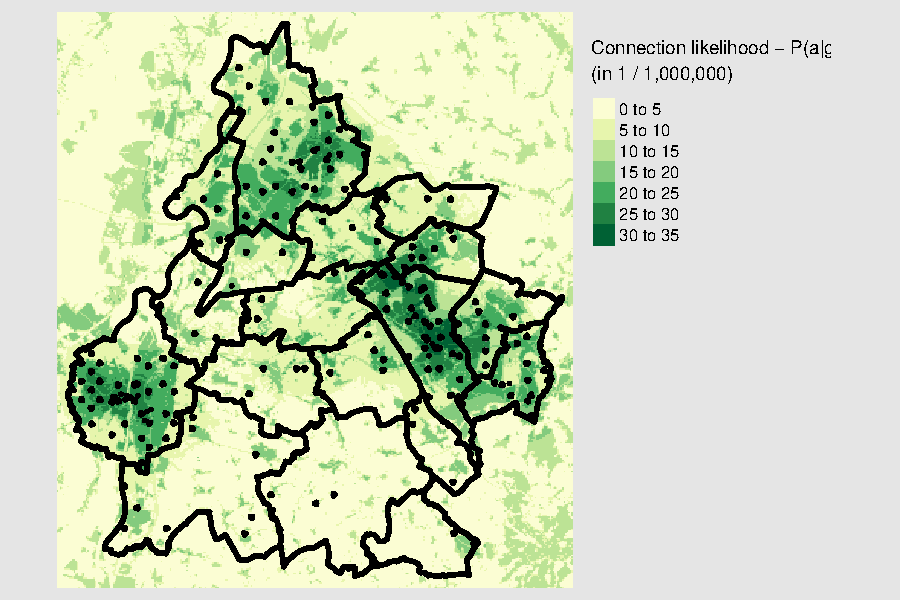
\includegraphics[width=0.46\linewidth]{mobvis-mobloc_files/figure-latex/unnamed-chunk-10-1}
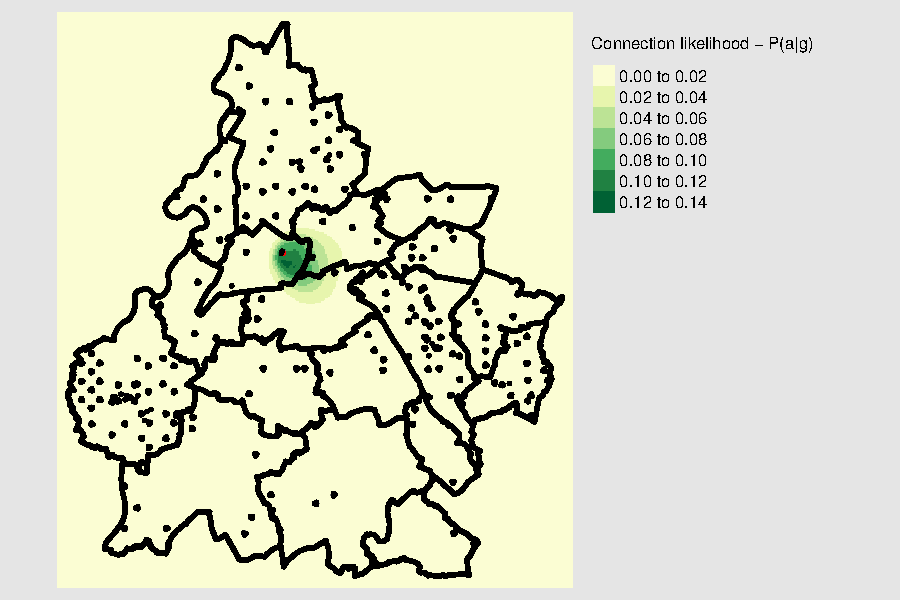
\includegraphics[width=0.46\linewidth]{mobvis-mobloc_files/figure-latex/unnamed-chunk-10-2}
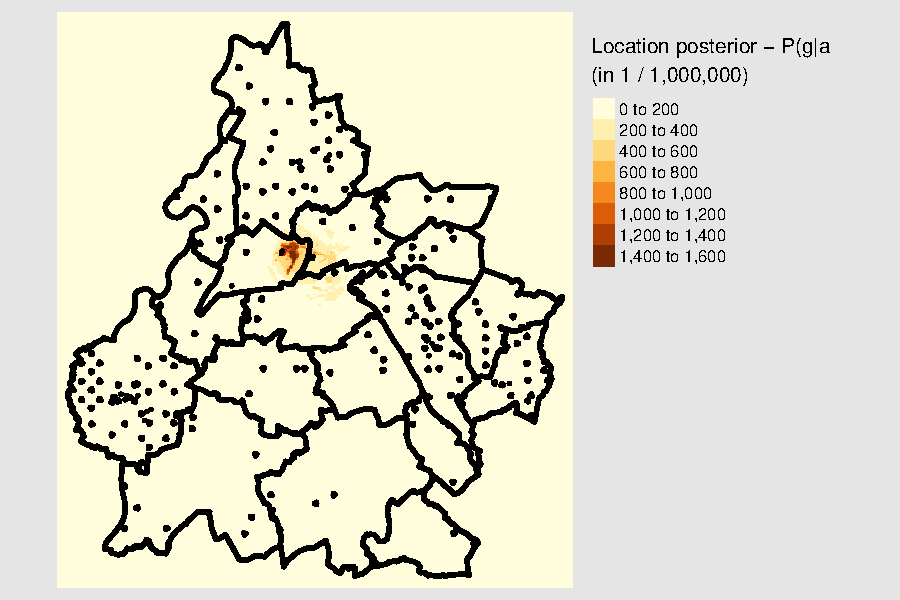
\includegraphics[width=0.46\linewidth]{mobvis-mobloc_files/figure-latex/unnamed-chunk-10-3}

Note that in these functions, the prior is a \texttt{raster} object
(parameter \texttt{rst}) whereas the likelihood and the posterior are
\texttt{data.table}s (parameter \texttt{dt}). The reason of these
formats is that the prior distribution is defined on the level of grid
tile; recall that the notation is P(g). The other two, the likelihood
(event location) and posterior distribution, are defined per grid tile
per cell, in mathematical notation P(a\textbar g) and P(g\textbar a)
respectively.

\hypertarget{references}{%
\subsection{References}\label{references}}

\begin{enumerate}
\def\labelenumi{\arabic{enumi}.}
\tightlist
\item
  Tennekes, Gootzen, Y.A.P.M., Shah, S.H. (2020) A Bayesian approach to
  location estimation of mobile devices from mobile network operator
  data, working paper, Statistics Netherlands, Heerlen.
\item
  Tennekes, M. (2020) mobloc: mobile location algorithms and tools,
  R-package
\item
  Salgado, D. et al.~(2018) Proposed elements for a methodological
  framework for the production of official statistics with Mobile Phone
  Data, ESSnet Big Data, WP5, Deliverable 5.3, Eurostat.
\item
  Pebesma, E., 2018. Simple Features for R: Standardized Support for
  Spatial Vector Data. The R Journal 10 (1), 439-446,
  \url{https://doi.org/10.32614/RJ-2018-009}
\item
  Robert J. Hijmans (2020). raster: Geographic Data Analysis and
  Modeling. R package version 3.3-13.
  \url{https://CRAN.R-project.org/package=raster}
\end{enumerate}

\end{document}
